% TODO: CITACAO DEPOIS DO CONCEITO
In the context of our research, we consider classes as the components

\section{Abstract}

Software modularization recovery algorithms automatically recognize a system's
modular structure by analyzing its implementation.
Due to the lack of well document software systems, though, the issue of testing
these algorithms is still underexplored, limiting both their adoption in the
industry and the development of better algorithms.
We propose to rely on software models to produce arbitrarily large test sets. In
this paper we consider three such models and analyze how similar the artifacts
they produce are from artifacts from real software systems.

\section{Introduction}

%   I want less time, so I hire more programmers
%   Thee project can consume more time, due to comunication costs between
% programmers.
%   Unless there is a good division of tasks
%
% (needn't be large)

One of the most obvious ways to reduce the time needed to develop or maintain a
software system is to assign more developers to it. When combined with poor
management, though, adding developers may in fact raise the development time,
due to the increasing communication cost between developers \cite{Brooks1995}.
Poor management may result in developers working on overlapping tasks, writing
duplicated code, and inadvertently breaking the code written by another
developer.

%The development and maintenance of large software systems is a big challenge for
%software engineering \cite{Northrop2006}. In order to reduce the development
%time of such a system, a tempting idea is to assign more developers for the
%project. 

In order to take advantage of a team of developers, therefore, a key issue is
the ability to decompose a system into weakly coupled modules, so that each
module is maintained by a distinct group of developers \cite{Parnas1972}.
Because of the weak coupling between modules, the need for communication between
groups of developers is reduced, and so is the development time.
 
The ability of decomposing a system into modules depends on global knowledge
about how its implementation components (e.g., functions, classes, variables)
interact. Often, specially in legacy systems, this information is not readily
available. Instead, it must be extracted from the system's source code. Even
then the task of finding modules may be overwhelming because of the large number
of components and interactions.

The task can be made easier by the use of software clustering algorithms, also
known as also known as architecture recovery algorithms \cite{Pollet2007}. They
automatically decompose a software system into weakly coupled modules by
analyzing the network of dependencies between its components.

% sw clustering is a task of reverse engineering \cite{Tonella2007}.

An important question for the adoption of a software clustering algorithm is
whether the decomposition it finds for a system is similar to a reference
decomposition for that system, i.e., a decomposition found by a group of
experienced developers. To answer this question one needs to test the algorithm
by applying it to a sample of systems with known reference decompositions, and
then compare the two decompositions for each system by means of a metric such as
MoJo \cite{Tzerpos1999} and EdgeSim \cite{Mitchell2001}.

Unfortunately there are few systems with known reference modularizations.
Furthermore, because it is costly to obtain reference modularizations
\cite{Koschke2000}, there are few empirical studies about software clustering
algorithms, most of them based on a couple of small and medium systems.

%  \begin{figure*}[!t]
%  \centering
%  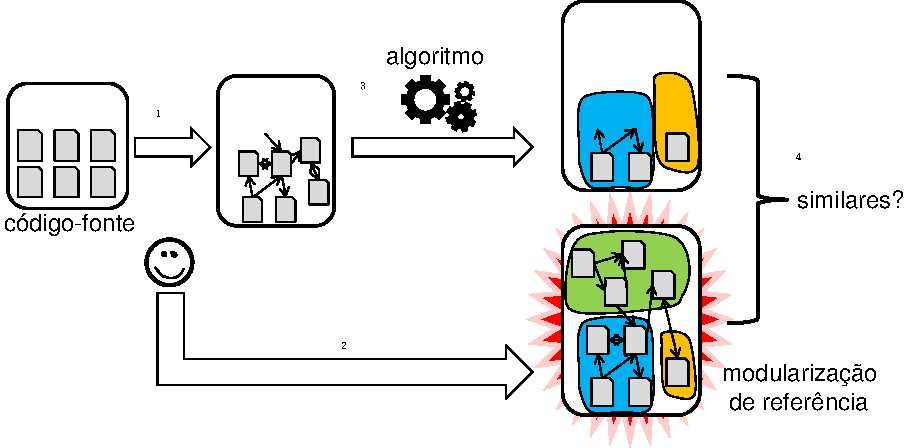
\includegraphics[width=1.0\textwidth]{diagram}
%  \caption{Evaluation of a software clustering recovery algorithm}
%  \label{fig:diagram}
%  \end{figure*}

In this research we propose to evaluate software clustering algorithms by
applying them to synthetic, i.e., computer generated, component dependency
networks with built-in decompositions. With this approach it is feasible to test
algorithms with arbitrarily large samples in a controlled manner.

Of course, it is desirable that the synthetic networks resemble networks
extracted from real software systems. Hence, in this paper, we describe a study
about three models that synthesize networks with built-in decompositions. We
show empirically that all three models are capable of synthesizing networks that
resemble software networks.

The remaining sections are organized as follows. .... Section 2, ...

%alike, resembling, exchangeable, indistiguible

%\section{Related Work}
%
%\section{Software Modularization Recovery: an Overview}
%Aka software architecture recovery, software architecture reconstruction,
%software clustering...
%It's an task of reverse engineering, as defined by Tonella \cite{Tonella2007}...
%DEFINITIONS
%external edge...

%\section{Software Networks and Software Clustering}
%
%directed graph, (un)weighted

\section{Software Networks}

The implementation of a software system can be viewed as a network of
interacting components. In a object-oriented system, for example, classes
interact with other classes through mechanisms such as inheritance and
aggregation. By abstract the particular mechanisms of interaction, it is
possible to build a network of dependencies between components, represented as a
directed graph. This kind of network is the input for many software clustering
algorithms \cite{Mancoridis1998,Anquetil1999,Tzerpos2000,Andritsos2005}.

In this paper we will study networks of dependencies between classes in
object-oriented systems. We will call any such a network a \emph{software
network}. 

%Define: Component. Component dependency network. Directed unweighted graph.
%Clustering based on dependencies.

Network theory research studies general properties of many types of networks by
using statistical analysis. In the last decade, it has been found that many
networks arising from sociology, biology, technology and other domains present
remarkable structural similarities. It has been shown that, in these networks,
the distribution of vertex degrees is a power law, i.e., the number of vertices
connected to $k$ edges, N($k$), is proportional to $k^{\-gamma}$, where $\gamma$
is a positive constant. These networks are called scale-free networks.

Network theory has been applied to software networks and it was shown that they
are also scale-free networks \cite{Myers2003,Valverde2003}.

%(in fact we can't argue the degree distribution is perfectly fit by a power law.
%Anyway, the distribution is much more assymetric than normal ou Poisson's)
%
%software indegree distribution (power law), outdegree distribution (not so power
%law)

\section{Network Models}

Many models were proposed to explain the formation of scale-free networks. These
models are simple algorithms that can be proven, either formally or empirically,
to synthesize networks that are scale-free. Most models, though, do not account
for modular structure, a feature present in some networks, in particular
software networks. In this section we present three models that generate
directed networks with built-in modular decompositions: BCR+, CGW and LR. 

%The first two models grow networks using a mechanism called
%preferential attachment CITE Barabasi, by which nodes with many edges tend to
%receive more edges in the process.

%\subsection{ER (Erdos-Renyi)}

%\subsection{Configuration model}
% take the most typical software system and steal its degree sequence

\subsection{BCR+}

The BCR model \cite{Bollobas2003} aims to model the network of hyperlinks
between web pages as a directed graph without modules. It was proven
analitically to generate scale-free networks. We have developed an extension to
this model, called BCR+, that adds modules to the construction of the network.
The model accepts the following parameters:

\begin{itemize}
\item number of vertices, $n$;
\item a graph, $G$;
\item three probabilities, $p$, $q$, and $r$, such as $p + q + r = 1$;
\item a probability, $mu$;
\item two real numbers, $din$ and $dout$.
\end{itemize}

In a network with modules, one can define a module dependency graph (MDG) as a
graph where the two following conditions hold: 

\begin{itemize}
\item each vertex represents a module in the original network; 
\item there is an edge from $M_1$ to $M_2$ in the MDG only if there is an edge
from $v_1$ to $v_2$ in the original network, where $v_1 \in M_1$ and $v_2 \in
M_2$.
\end{itemize}

The BCR+ model generates networks whose MDG is equal to $G$ by adding vertices
and edges to an initial network until it reaches $n$ vertices. The initial
network is isomorphic to $G$: it contains one vertex for each module and one
edge for each edge in $G$, connecting vertices whose corresponding modules are
connected. Thus, the MDG for the generated network is equal to $G$ from the very
beginning.

After that, the algorithm consists of successive applications of one out of
three operations on the network: (1) adding a vertex with an outgoing edge; (2)
adding a vertex with an ingoing edge; (3) adding a edge between existing
vertices. In operation 3, the edge can connect either vertices that belong
to the same module or vertices in distinct modules. 

The choice of the vertices that will be connected by a new edge, although
non-deterministic, is not fully random. The probability that a particular vertex
v is choosen, P($v$), is proportional to a function of the in-degree or the
out-degree of the node. We say that we choose a vertex within a set of vertices
$S$ according to a function f if

$$
  P(v) ~=~ \frac{ f(v) }{ \sum_{v \in S, f(v)} }.
$$

The denominator is a normalizing factor that assures that the probabilities sum
to 1.

Before we present the algorithm in detail, using pseudo-code, we must define
some functions:

%Let V be the set of vertices in the network being generated. This
%set grows as the algorithm is executed. Being v a vertex, we define the
%following three functions:

\begin{itemize}

\item in-degree(v): the number of edges that enter in the vertex v;

\item out-degree(v): the number of edges that leave the vertex v;

\item module(v): the module to which the vertex v belongs;

\item out-neighbors(v): the set of all vertices that are connected to the vertex
v by an edge starting in v.

\item same-module(v): the set of all vertices that are in the same module as the
vertex v, except for v itself and vertices in out-neighbors(v).

\item other\_modules(v): the set of all vertices that are in modules that are
connected to v's module (in the graph G) by an edge starting in v's module,
except for vertices in out-neighbors(v).

\end{itemize}

After the initial network is created, the algorithm proceeds as follows:

\begin{figure*}
\begin{verbatim}
while the number of nodes in the network is less than n:
  choose one of the operations according to probabilities (p, q, r)
  operation 1: (add a vertex with an outgoing edge)
    choose a vertex w within V according to f(x) = din + in-degree(x)
    add a new vertex, v, to module(w)
    add an edge from v to w
  operation 2: (add a vertex with an ingoing edge)
    choose a vertex w within V according to f(x) = dout + out-degree(x)
    add a new vertex, v, to module(w)
    add an edge from w to v
  operation 3: (add an edge between two existing vertices)
    choose a vertex v within V according to f(x) = dout + out-degree(x)
    choose a case according to probabilities (mu, 1 - mu)
    case 1: (distinct modules)
  	  choose a vertex w within other\_modules(v) according to f(x) = din + in-degree(x)
      add an edge from v to w
    case 2: (same module)
      choose w within same-module(v) according to f(x) = din + in-degree(x)
      add an edge from v to w
\end{verbatim}
\end{figure*}

We can see that the probabilities $p$, $q$, and $r$ control how often each
operation is performed. Because the operation associated with probability $r$
does not add any vertices, greater values of $r$ imply more edges in the
resulting network. It is easy to see that nodes connected to many ingoing edges
are more likely to get another ingoing edge, and the same reasoning can be
applied to outgoing edges. The parameter $din$ can alleviate the handicap by
providing a ``base in-degree'' that is applied to all vertices when computing
the probabilities. Consider two vertices, $v_1$ with in-degree 4, and $v_2$ with
in-degree 8. If $din = 0$, $v_2$ is twice more likely to receive a new incoming
edge; if, otherwise, $din = 4$, $v_2$ is only $\frac{3}{2}$ more likely to
receive the edge.

The parameter $mu$ controls the proportion of edges between vertices in distinct
modules. Lower values of $mu$ lead to networks with weakly coupled modules.

The BCR+ model is a growth model, meaning that the network is generated vertex
by vertex, growing from an initial network. It can, therefore, simulate the
evolution of a software network. Moreover, it can simulate the evolution of a
software system subject to constraints in module interaction, as is the case
with top-down system design methodologies CITE.

%* Add a node with ongoing edge. With probability p, a new vertex is added to the network, together with an
%edge from the new vertex to an existing vertex, chosen preferentially according
%to .... Considering din = 0, this means that a vertex with indegree = 8 is
%twice more likely to receive the edge than a vertex with indegree = 4. The
%parameter din can be used to alleviate the handicap. (If din = 4, the first
%vertex will only be 3/2 more likely to receive the edge). The new vertex is
%put on the same cluster as the old vertex.
%
%* Add a node with ingoing edge. With probability q, a new vertex is added to the network, together with an
%edge from an existing vertex, chosen preferentially accordingly to dout +
%outdegree, to the new vertex. The new vertex is put on the same cluster as the
%old vertex. This case is similar to the previous case.
%
%* Add an edge. With probability r, a new edge is added between two vertices, v and w. v is
%chosen according to .... After that, with prob X, w is chosen from one of the
%modules connected to v's module, else it's chosen from v's own module. In any
%case, the exact choice is made according to ...
%
%It's a growth model, that is, it can take as input an existing network and
%evolve it.
%
%TODO: Argument: why the imposed modules are natural modules?

\subsection{CGW}

The CGW model \cite{Chen2008} was proposed to model the evolution of software
systems organized in modules. It was proven formally to generate scale-free
networks.  It accepts the following parameters:

\begin{itemize}
\item Number of vertices, n;
\item Number of modules, m;
\item Probabilities p1, p2, p3, p4, summing 1;
\item Natural numbers e1, e2, e3, e4;
\item Constant $\alpha$, with $\alpha \ge -1$
\end{itemize}

Just like BCR+, this is a growth model. Its initial network is composed of two
vertices belonging to the same module and a directed edge between them. The
remaining $m - 1$ modules are initially empty. 

After that, the algorithm consists of successive applications of one out of four
operations on the network, which are chosen according to probabilities p1, p2,
p3, and p4: 
(1) adding a vertex with e1 outgoing edges; 
(2) adding e2 edges;
(3) rewiring e3 edges;
(4) removing e4 randomly chosen edges.

Whenever an edge is added from a vertex $v$ to a vertex $w$ (operations 1, 2,
and 3), $v$ is chosen randomly, and $w$ is chosen according to the following
probability function:

$$
  P_v(w) ~=~ \frac{ f_v(w) }{ \sum_{w \in S, f_v(w)} },
$$

where

$$
f_v(w) = 1 + degree(w) \cdot (1 + \alpha), if module(w) = module(v)
, 1 + degree(w), otherwise
$$

Because the original paper did not provide an implementation for the model, we
now present the pseudo-code for our implementation:

\begin{figure*}
\begin{verbatim}
while the network has less than n vertices:
  choose operation (p1, p2, p3, p4)
  operation 1: (adding a vertex with e1 outgoing edges)
    create a new vertex v and add it to a randomly chosen module
    do e1 times:
      choose a vertex w according to f_v(w)
      add an edge from v to w
  operation 2: (adding e2 edges)
    do e2 times:
      choose a vertex v randomly
      choose a vertex w according to f_v(w)
      add edge from v to w
  operation 3: (rewiring e3 edges)
    do e3 times:
      choose a vertex v randomly
      choose an edge e randomly within edges that start in v
      choose w according to f_v(w)
      remove e
      add an edge from v to w
  operation 3: (removing e4 edges)
    do e4 times:
      remove and randomly chosen edge
\end{verbatim}
\end{figure*}

Unlike BCR+, this model does not allow constraints on the connection between
modules, however it accounts for the rewiring and the removal of edges. 

\subsection{LF}

The LF model \cite{Lancichinetti2009} is a very flexible model that can
generated weighted directed networks with overlapping modules, that is, in which
a vertex can belong to more than one module. Unlike the previous models, this is
not a growth model: all vertices are generated at once and then the edges are
added.

There is also a special version of the model in which the edges weights are
discarded and the modules are non overlapping. We used the original
implementation of this version, available at
\url{http://santo.fortunato.googlepages.com/inthepress2}. It accepts the following
parameters:

\begin{itemize}
\item number of nodes, $n$;
\item average in-degree, $k$, with $k < n$;
\item maximum in-degree, $max_k$, with $max_k \ge k$ and $max_k < n$;
\item mixing parameter, $\mu$, with $0 \le \mu \le 1$;
\item minus exponent for the degree distribution, $\gamma$;
\item minus exponent for the module size distribution, $\beta$;
\item minimum module size, $min_m$;
\item maximum module size, $max_m$, with $max_k \ge min_k$;
\end{itemize}

The sizes of the modules are selected from a power law distribution with
exponent $-\beta$. The mixing parameter, $\mu$ is the proportion of edges in the
network that connect vertices from distinct modules. In this model, some
combinations of parameter values are unfeasible. For example, if $n = 100$ then
$min_m$ cannot be 60 (otherwise there would be modules smaller than the minimum
module size).

%%%%%%%%%%%%%%%%%%%%%%%%%%%%%%%%%%%%%%%%%%%%%%%%%%%%%%%%%%%%%%%%%%%%%%%%%%%%%%
%%%%%%%%%%%%%%%%%%%%%%%%%%%%%%%%%%%%%%%%%%%%%%%%%%%%%%%%%%%%%%%%%%%%%%%%%%%%%%
%%%%%%%%%%%%%%%%%%%%%%%%%%%%%%%%%%%%%%%%%%%%%%%%%%%%%%%%%%%%%%%%%%%%%%%%%%%%%%

\section{Characterization of Software Networks}

Our research hypothesis is that at least one of the presented models can
synthesize networks that resemble software networks. A central issue, thus, is
how to measure similarity between networks. In order to be useful, a similarity
metric must be able to differentiate between software and non-software networks.
In this section we present such a metric, together with an experiment that
evaluates its usefulness by applying it to both software and non-software
networks. %Then we show a classification model 

%%%%%%%%%%%%%%%%%%%%%%%%%%%%%%%%%%%%%%%%%%%%%%%%%%%%%%%%%%%%%%%%%%%%%%
\subsection{Similarity Between Networks}

In a recent work, Milo et al. \cite{Milo2002} proposed to characterize networks
by analyzing their triad concentration. A triad is a network with three vertices
in which all vertices are connected. There are only 13 distinct triads, one for
each configuration of directed edges, as shown in Figure \ref{fig:triads}.

CITE igraph

\begin{figure*}[!t]
\centering
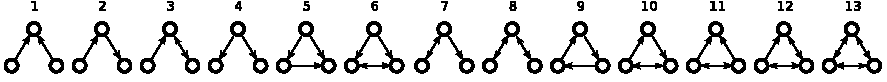
\includegraphics[width=1.0\textwidth]{triads}
\caption{Triads (id vs. graph. reprs.)}
\label{fig:triads}
\end{figure*}

By counting how many times each triad appears in a network, one can build a
triad concentration profile (TCP), which is a vector with 13 numbers that
summarize the local structure of the network. Figure \ref{fig:profiles} shows
the TCP for networks from distinct domains.

Following the work by Milo et al. \cite{Milo2004}, similarity between two
networks can be measured by computing Pearson's correlation coefficient between
the corresponding TCPs, which yields a value between -1 (most dissimilar) and 1
(most similar):

$$
\mathrm{sim}(a, b) ~=~ \mathrm{cor}(\mathrm{TCP}(a), \mathrm{TCP}(b))\mathrm{,}
$$

where $a$ and $b$ are networks, TCP($x$) is the triad concentration profile for
network $x$, and cor($x$, $y$) is Pearson's correlation coefficient.

% Word adjacency network: word Y follows word X => X->Y
\begin{figure}[!t]
\center
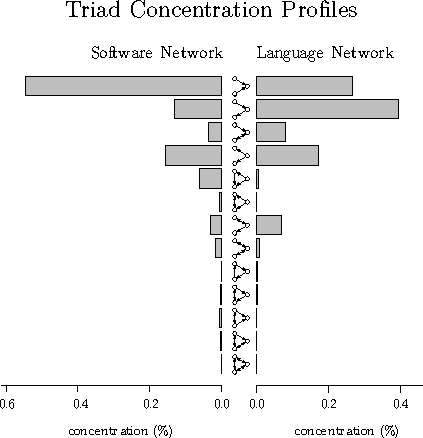
\includegraphics{tcp}
\caption{Triad concentration profiles (TCP) for two networks. On the left,
network extracted from the software system JabRef (see the Appendix). On the
right, word adjacency network for the Japanese language \cite{Milo2004}.}
\label{fig:profiles}
\end{figure}

%%%%%%%%%%%%%%%%%%%%%%%%%%%%%%%%%%%%%%%%%%%%%%%%%%%%%%%%%%%%%%%%%%%%%%
\subsection{Data Set}

To support the evaluation of the metric, we have collected 131 networks. The
networks are described in detail in the Appendix.

\textbf{Software networks}. We have collected 65 software systems written in
Java, with size ranging from 111 to 35,363 classes. Java was chosen for being a
popular programming language in which many open source systems have been
written. The software networks, representing dependencies between classes, were
extracted with the tool Dependency Finder CITE.

\textbf{Non-software networks}. We have collected 66 networks from distinct
domains, such as biology, sociology, technology, and linguistics. These networks
are freely available on the Internet and have been used in previous researches.
CITE

% S-score

%%%%%%%%%%%%%%%%%%%%%%%%%%%%%%%%%%%%%%%%%%%%%%%%%%%%%%%%%%%%%%%%%%%%%%
\subsection{Evaluation of the Similarity Metric}

In order to evaluate the similarity metric, we measured the similarity between
the networks in the data set. A suitable metric must fullfil two conditions: (i)
it must yield high similarity between software networks, and (ii) it must yield
lower similarity between software networks and networks from other domains.

Using the data set we can define S-score, a metric that represents how much a
particular network resemble software networks. It is defined as the average
similarity between the network and a sample of software networks:

$$
\mathrm{S\mbox{-}score}(a) = \frac{
\sum_{s \in S} \mathrm{sim}(a, s)
}{|S|} \mathrm{,}
$$

where $S$ is the set of sample software networks, and $|S|$ is the number of
networks in $S$. In this work we use the full software data set consisting of 65
software networks as our sample.

We measured the S-score for each software network, which ranged from 0.83 to
0.98. The average S-score was 0.97 and the standard deviation, 0.03. The high
average S-score and the low standard deviation show that the metric successfully
characterizes software networks by capturing common structural patterns

TODO: Boxplot by network class (software, metabolic, neural, social etc.)

Then we measured the S-score for each non-software network. The majority of the
networks (X\%) had a S-score lower than 0.83, which is the lowest S-score for
software networks in the sample. Some networks, showing friendship between
students, showed negative S-score, meaning that they are very different from
software networks.

Two networks, though, showed high S-score, above 0.83. The network of links
between blogs on politics showed S-score 0.97. The neural network of the worm
C. Elegans also showed a high S-score (0.88). Further investigation is needed
in order to discover the reasons behind these high S-scores and whether
auxiliary metrics can differentiate these networks from software networks.

\subsection{A Network Classification Model} \label{sec:classmodel}

Although the S-score of a network tells how close it is from software networks,
it does not tell whether a network is close enough that it can be considered
software-like. What is needed is a binary classification model that
distinguishes software-like networks from the other networks. The distinction
can be made by choosing a suitable S-score threshold. Networks with S-score
below the threshold are considered dissimilar from software networks; only
networks with S-score above the threshold are considered software-like. 

As we have shown on the previous section, there are non-software networks with
high S-scores, hence it is impossible to build a perfect classification model,
regardless of the threshold. Nonetheless, such a model can be evaluated by its
precision and recall. Consider a data set with both software and non-software
networks. Let $S$ be the set of all software networks, and $L$ the set of all
networks that were classified by the model as software-like. The precision of
the model is

$$
\mathrm{precision}: ~\frac{S \cap L}{L},
$$

and the recall is

$$
\mathrm{recall}: ~\frac{S \cap L}{S}.
$$

Increasing the threshold has the effect of reducing the recall, because fewer
software networks are classified as software-like. Decreasing the threshold has
the effect of reducing the precision, since more non-software networks are
classified as software-like. 

The choice of a proper threshold, thus, depends on whether it is more important
to have high precision or high recall. Because our research hypothesis is that
networks synthesized by the presented models are software-like, higher precision
means a stronger test, as fewer networks are classified as software-like.

To get 100\% precision, the threshold needs to be 0.98, so the non-software
network with highest S-score is below the threshold. The recall in this case,
though, would be too low, because most software networks would be misclassified.
So we chose the value 0.88, that is immediatly greater than the second greater
non-software network S-score. With this value, we have both a high recall
(95.4\%) and a high precision (96.9\%).

%threshold 0.88: 2/66 non-sw misclassified, 3/65 sw misclassified
%precision: 62 / 64
%recall: 62 / 65

%%%%%%%%%%%%%%%%%%%%%%%%%%%%%%%%%%%%%%%%%%%%%%%%%%%%%%%%%%%%%%%%%%%%%%%%%%%%%%
%%%%%%%%%%%%%%%%%%%%%%%%%%%%%%%%%%%%%%%%%%%%%%%%%%%%%%%%%%%%%%%%%%%%%%%%%%%%%%
%%%%%%%%%%%%%%%%%%%%%%%%%%%%%%%%%%%%%%%%%%%%%%%%%%%%%%%%%%%%%%%%%%%%%%%%%%%%%%

\section{Evaluation of Network Models}
% v.  differentiate, differ; distinguish; contrast; discern 

In the previous section it was shown that many networks, although scale-free,
can be distinguished from software networks by a simple classification model
based on triad concentration profiles. In this section we show empirically that
the three network models previously presented synthesize networks that are
indistinguishable from software networks.

The experiment consists of synthesizing networks using many combinations of
parameters from the three models, and then classifying each network as
software-like or non software-like. After that, we present rules for the choice
of parameter values that lead to software-like networks.

\subsection{Synthetic Data Set}

We want to investigate if, with a proper choice of parameters, a model is
capable of synthesizing a network that resembles software networks. Because the
possible combinations of parameter values are infinite, we have set the number
of vertices to 1000 and then varied the remaining parameters in discrete steps.
In this section we describe the combinations of parameters values used for each
model.

\subsection{BCR+ networks}

We have chosen five different module dependency graphs, which where extracted
from actual dependencies between archives of five different software systems of
our sample: GEF (2 archives), iBATIS (4 archives), MegaMek (8 archives),
findbugs (16 archives), and zk (32 archives). 
%The module dependency networks are shown on Figure \ref{fig:architectures}. 
%\begin{figure*}[!t]
%\centering
%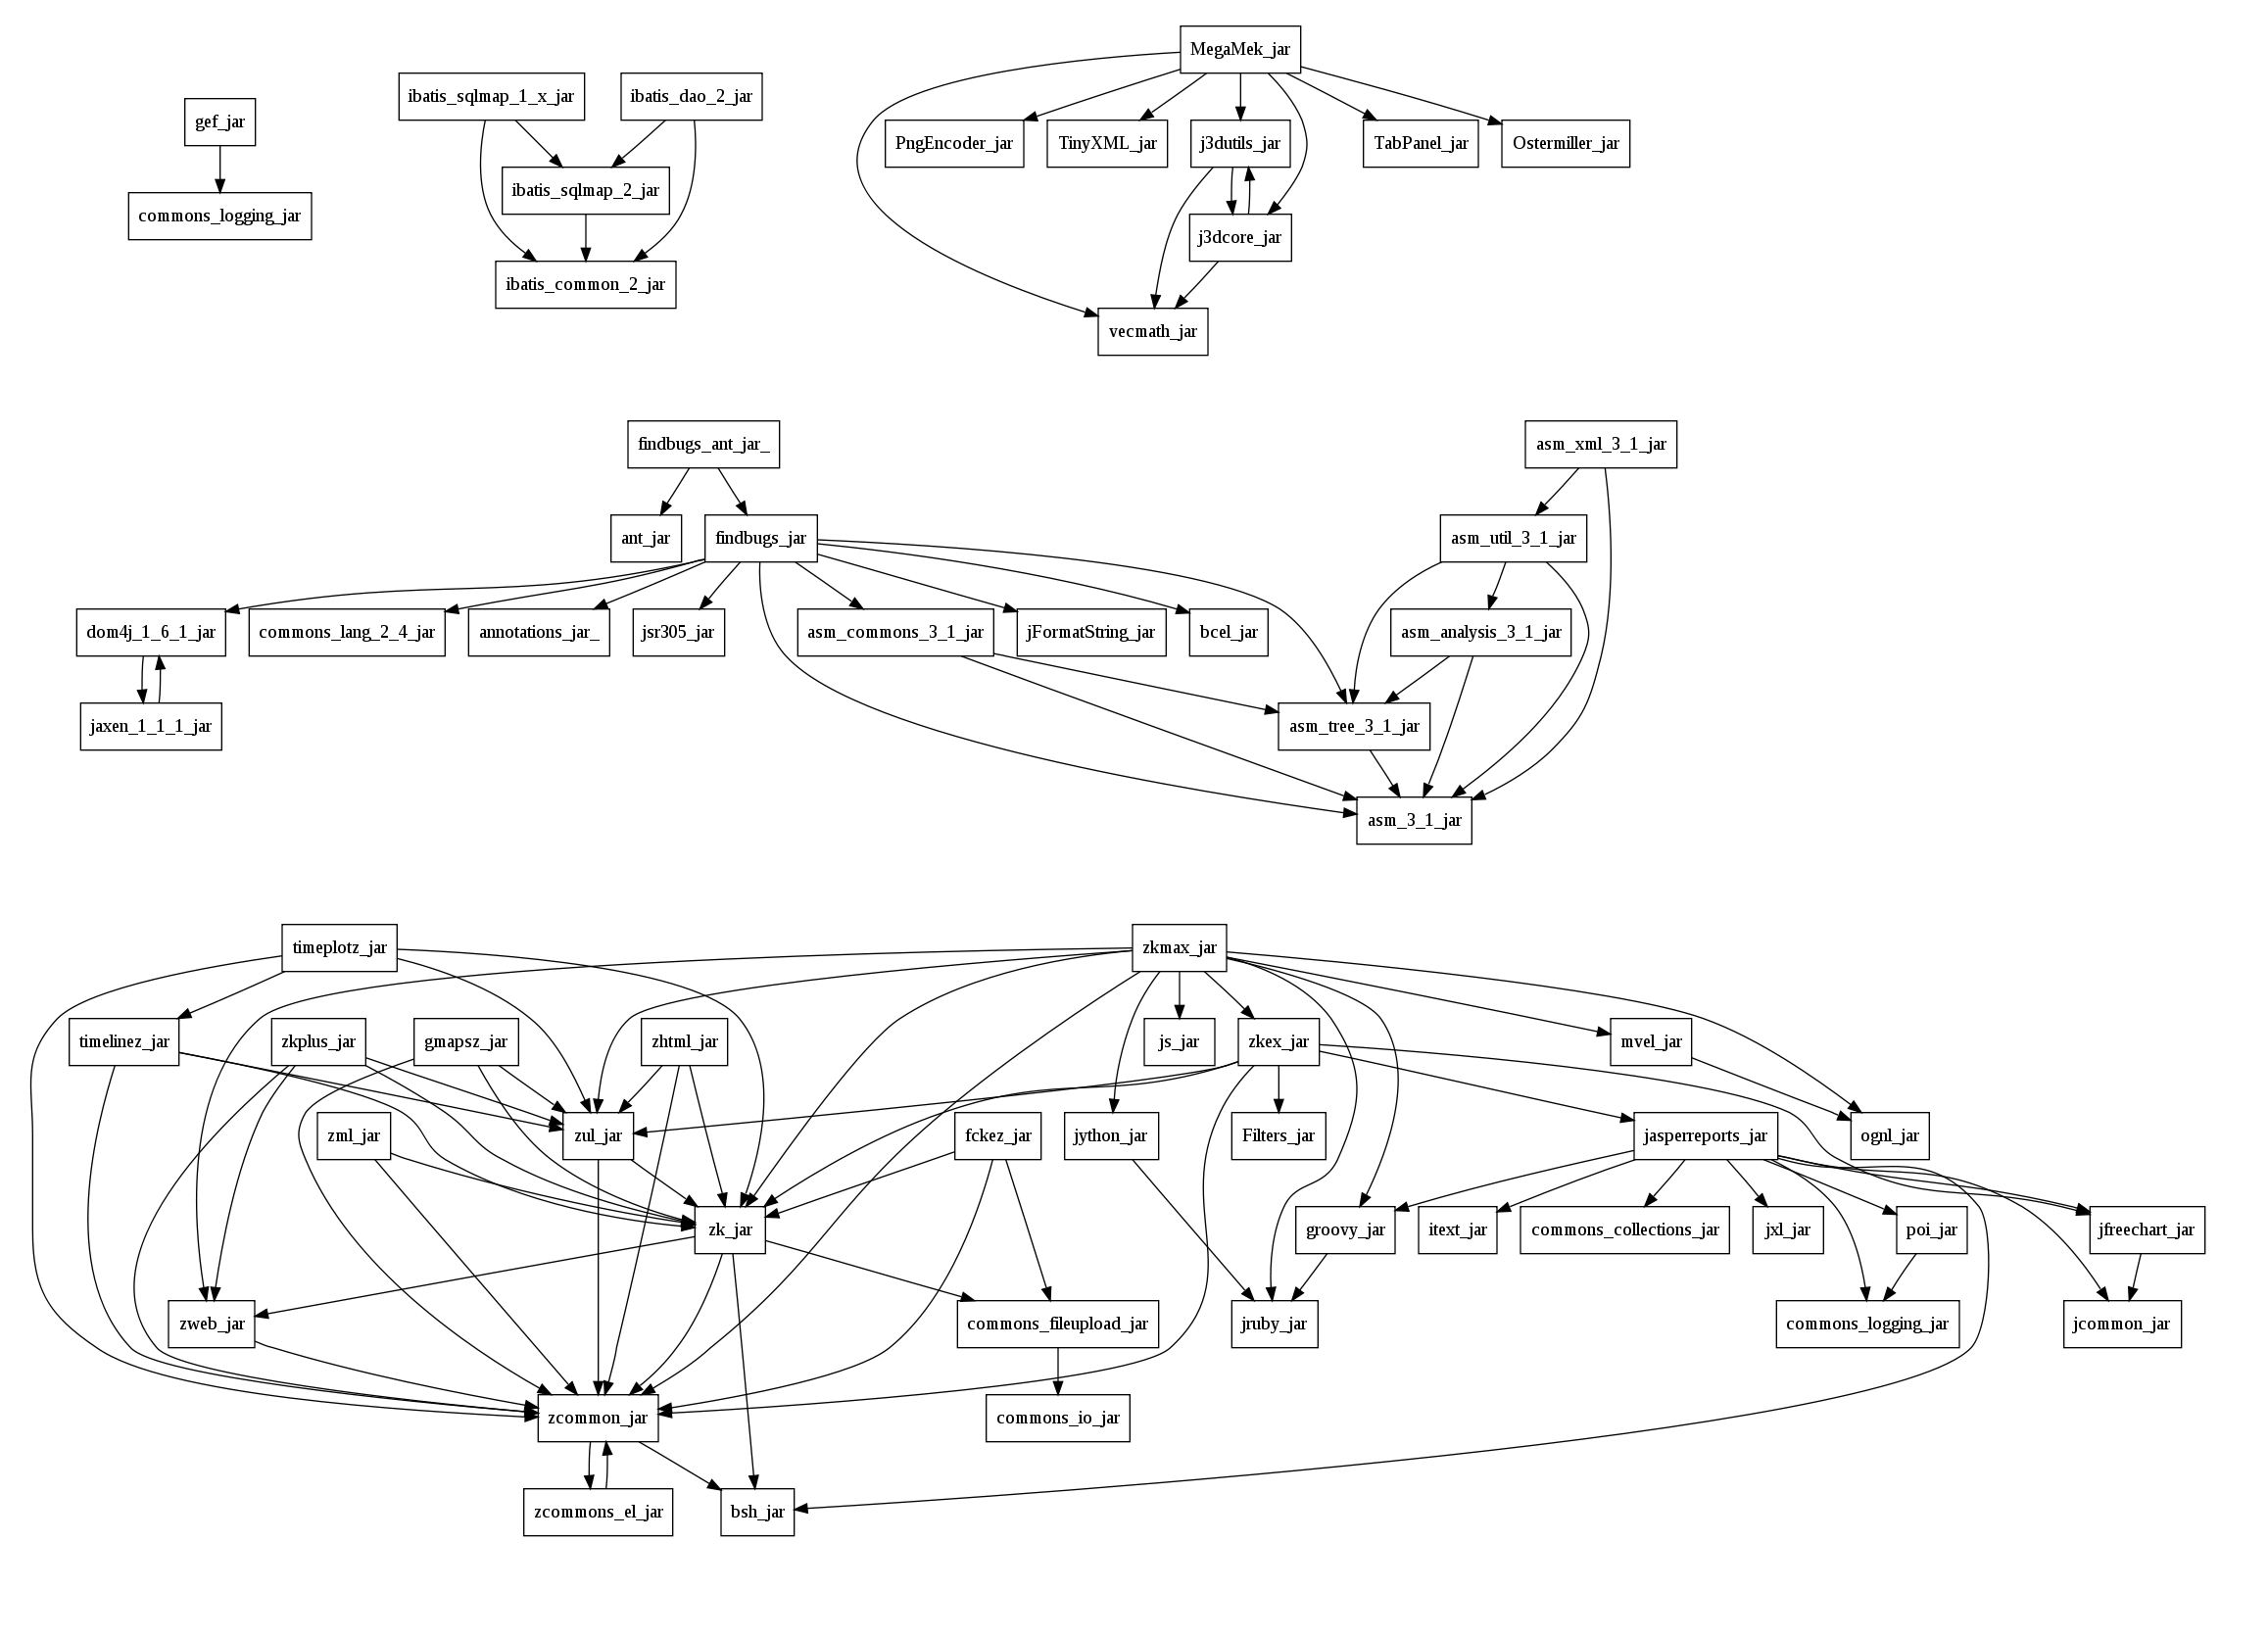
\includegraphics[width=1.0\textwidth]{architectures}
%\caption{Module dependency graphs}
%\label{fig:architectures}
%\end{figure*}

For the remaining parameters, the following values were given:

\begin{itemize}
\item $p, q, r \in \{0.0, 0.2, 0.4, 0.6, 0.8, 1.0\}$, with $p + q + r = 1$ and
$p + q > 0$;
\item $din, dout \in \{0, 1, 2, 3, 4\}$;
\item $\mu \in \{0.0, 0.2, 0.4, 0.6\}$.
\end{itemize}

We chose $p + q > 0$ because otherwise no node would be added after the
creation of the initial network. We also avoided large values for $\mu$ in
order to ignore networks with highly-coupled modules. 

In total, 9,500 BCR+ networks were synthesized.

\subsection{CGW networks}

The parameters values were chosen as such:

\begin{itemize}
\item $p1, p2, p3, p4 \in \{0.0, 0.2, 0.4, 0.6, 0.8, 1.0\}$, with $p1 > 0$ and
$p1 + p2 + p3 + p4 = 1$;
\item $e1, e2, e3, e4 \in \{1, 2, 4, 8\}$;
\item $\alpha \in \{-1, 0, 1, 10, 100, 1000\}$;
\item number of modules: $m \in \{2, 4, 8, 16, 32\}$.
\end{itemize}

Notice that $e_i$ has no effect when $p_i = 0$; in this case $e_i$ was just set
to zero.

In total, 38,790 CGW networks were synthesized.

\subsection{LF networks}

The following values were chosen:

\begin{itemize}
  \item mixing parameter: $\mu \in \{0.0, 0.2, 0.4, 0.6\}$;
  \item degree exponent distribution: $\gamma \in \{2.18, 2.70, 3.35\}$;
  \item module size distribution: $\beta \in \{0.76, 0.99, 1.58\}$;
  \item average degree: $k \in \{5, 10, 15, 25\}$;
  \item maximum degree: $max_k \in \{58, 157, 482\}$;
  \item minimum module size: $min_m \in \{1, 10, 273\}$.
\end{itemize}

In order to choose these values, we analyzed software networks from our sample
with approximately 500 to 2,000 nodes, so no network was much bigger or much
smaller than the synthetic networks. We computed the exponents for the degree
and module size distributions using the maximum likelihood estimation method
\cite{Clauset2007}, and then chose the minimum, median and maximum values. For
$k$, $maxk$, and $min_m$, the values extracted from the software networks were
divided by the number of nodes in the network and then multiplied by 1000. We
then selected the minimum, median and maximum values. The parameter $max_m$ was
left unbound to avoid impossible combinations of parameters.

In total, 1,296 LF networks where synthesized.

\subsection{Results}
% This subsection needn't to be big. It's just numbers.

Each synthesized network was classified as software-like or non software-like,
using the classification model presented in section \ref{sec:classmodel}. The
results are summarized in Table \ref{tab:results}. 

\begin{table}
\caption{Results for the classification of synthetic networks}
\centering
\begin{tabular}{|l|l|}
\hline
Model & Networks classified as software-like \\
\hline 
\hline
BCR+ & 21.18\% \\ % 2012 / 9500
\hline
CGW  & 19.40\% \\  % 7524 / 38790
\hline
LF   & 31.25\% \\ %  405 / 1296
\hline
\end{tabular}
\label{tab:results}
\end{table}

All models synthesized both software-like and non software-like networks. The
proportion of software-like networks was greater than 19\% for all models,
discarding the possibility that this result was obtained by pure chance.

%Show some graphs: histogram of average correlations for each model.
%\ref{fig:histograms}
%\begin{figure*}[!t]
%\center
%
%\subfigure[CGW]{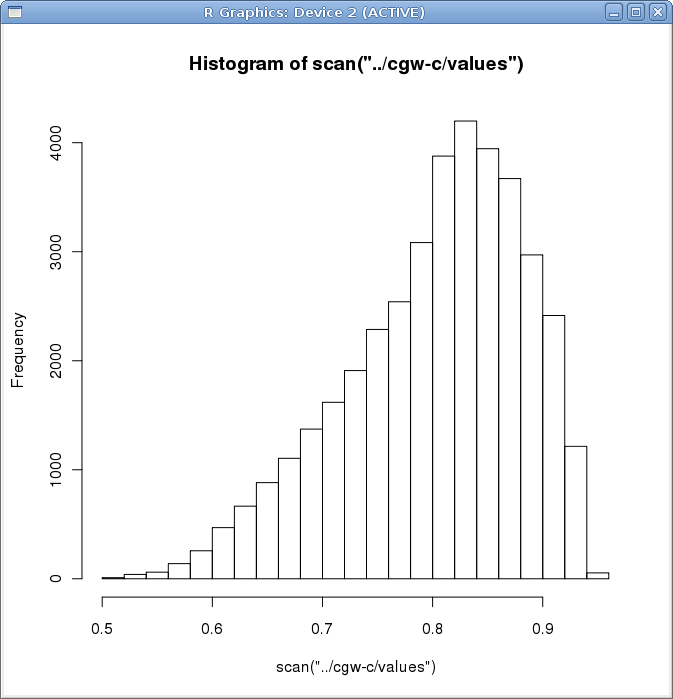
\includegraphics[width=1.0in]{hist-cgw}}
%
%\subfigure[BCR+]{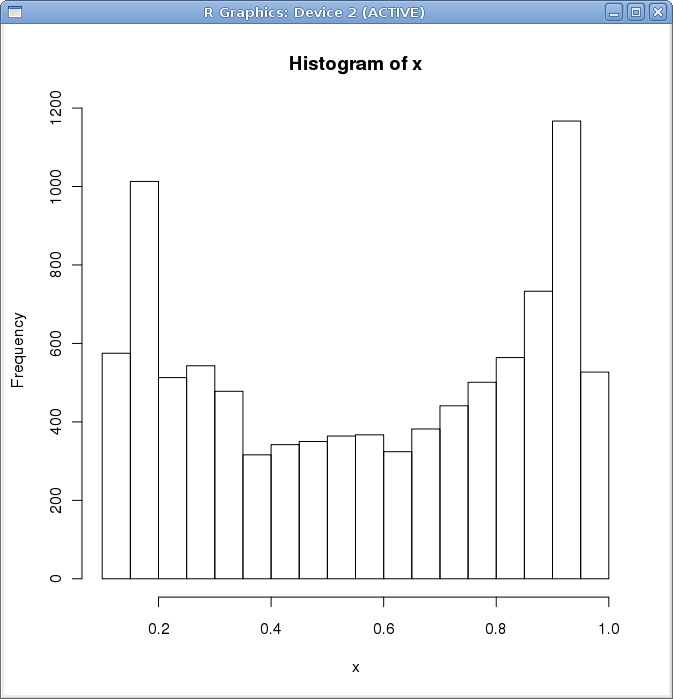
\includegraphics[width=1.0in]{hist-bcr}}
%
%\subfigure[LF]{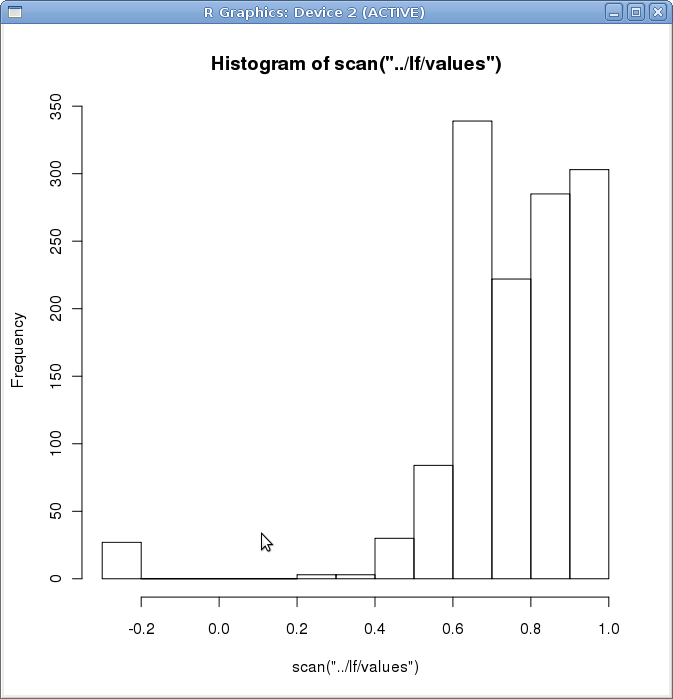
\includegraphics[width=1.0in]{hist-lf}}
%
%\caption{Triad profiles}
%\label{fig:histograms}
%\end{figure*}

Of course, this result is of little practical value unless there is a
relationship between parameter values and S-score. For the purpose of this
research, it is important to know which values are more likely to lead to
software-like networks.

The algorithm 1R from data mining was used to help discover such relationship.
It analyzes the parameters and the classification of each network and finds a
rule that relates the value of one single parameter with the classification. We
are interested in rules for networks classified as software-like and in the
accuracy of these rules, i.e., the proportion of networks that are correctly
classified. The rules found by 1R are shown in Table \ref{tab:rules}.

\begin{table}
\caption{Rules for predicting the classification of a synthetic network. S
stands for software-like and N stands for non software like.}
\centering
\begin{tabular}{|l|l|l|}
\hline
Model & Rule & Accuracy \\
\hline 
\hline
\multirow{2}{*}{BCR+}
     & $\alpha \ge 0.7 \Rightarrow S$ & \multirow{2}{*}{82.4\%}  \\ 
     & $\alpha < 0.7 \Rightarrow N$ & \\ 
\hline
\multirow{2}{*}{CGW}
     & $p_1 \ge 0.5 \Rightarrow S$ & \multirow{2}{*}{82.3\%} \\  
     & $p_1 < 0.5 \Rightarrow N$ & \\  
\hline
\multirow{2}{*}{LF}   
     & $\gamma \ge 2.44 \Rightarrow S$ & \multirow{2}{*}{78.9\%} \\ 
     & $\gamma < 2.44 \Rightarrow N$ & \\ 
\hline
\end{tabular}
\label{tab:rules}
\end{table}

The rules are very simple and, thus, easy to follow. Despite their simplicity,
they have high accuracy, approximately 80\% in all models.  
%These rules allow one to know if a particular combination of parameter values
%is likely to lead to software-like networks.

%\subsection{Parameter-Based Classification Models}
%
%1R

%Naive Bayes

%\subsection{Homogeinity}
%
%Pick realistic networks from a model. Are they similar to each other? (see
%standard deviation) In other words: do the parameters make a difference?
%
%Are they similar to networks generated by the other models? In other words: are
%the models equivalent?

%\section{Threats to validity}
%
%% External validity (EV): can it be generalized?
%
%%Structural information isn't enough for a expert do produce a
%%decomposition (s/he may use data such as names and external documentation). 
%%
%%Even when considering only structural information, is it true
%%that experts would find a decomposition similar to the reference decomposition
%%imposed by the model?
%
%We generated only one network for each set of parameters. (as we've shown, some
%parameters are redundant as they do not change significantly the realism)
%
%Some clustering algorithms use weights and they weren't studied here.
%
%EV: We've only studied 65 systems, which is not that much.
%
%We only studied object-oriented systems implemented in Java. Maybe the results
%would be different if we studied systems implement in other languagens or using
%other paradigms. The choice of a particular technique for extracting
%dependencies (static analysis) may also have impact on the structure of the
%networks.
%
%% Koschke says that experts decompositions vary by no more than 80? percent.

\section{Conclusion and Future Work}
% revised 2009-09-03

We have shown empirically that network models found in the literature can
synthesize networks that resemble the network of dependencies between classes in
object-oriented systems. This result supports the use of synthetic networks in
the evaluation of software clustering algorithms.
%that operate on class dependency networks. 

The use of synthetic data is common in distributed computing research, but still
underexplored in software engineering research. Because many reverse engineering
tasks rely on dependency data, we expect this work to have impact beyond the
software clustering community.

%Although the use of models and synthetic data is somewhat common in distributed
%computing research, it is underexplored in software engineering research. We
%expect this work to contribute to explore t
%common in distributed computing research, simulation is underexplored
%in software engineering. This work opens a door to the usage of simulation in
%the field of reverse engineering of software in order to evaluate RE 
%algorithms.

We accept that it is important to evaluate the algorithms with real software
networks, but we argue that the use of synthetic networks in a complementary
manner can give researchers new insights about the algorithms. First, the use of
models allows the creation of large test sets, thus diminishing the small sample
effects. Moreover, the networks are created in a controlled way, according to
model parameters, so it is possible to study the behavior of the algorithms with
different parameter values.

In a future work, we intend to use synthetic networks in the evaluation of
software clustering algorithms that were previously studied with real networks
\cite{Wu2005}. After that we will be able to compare the results obtained by
the approaches.

\appendix %{Network Data Set}

This appendix lists the networks used in this work.

\subsection{Software Networks}

Systems hosted by SourceForge (\url{http://sourceforge.net/}):
\begin{itemize}
\item AbaGuiBuilder-1.8
\item alfresco-labs-deployment-3Stable
\item aoi272
\item stendhal-0.74
\item battlefieldjava-0.1
\item checkstyle-5.0
\item dom4j-1.6.1
\item findbugs-1.3.8
\item freetts-1.2.2-bin
\item ganttproject-2.0.9
\item geoserver-2.0-beta1-bin
\item geotools-2.5.5-bin
\item gfp\_0.8.1
\item hibernate-distribution-3.3.1.GA-dist
\item hsqldb\_1\_8\_0\_10
\item iBATIS\_DBL-2.1.5.582
\item iReport-nb-3.5.1
\item JabRef-2.5b2-src
\item jailer\_2.9.9
\item jalopy-1.5rc3
\item jasperreports-3.5.2-project
\item jfreechart-1.0.13
\item pentaho-reporting-engine-classic-0.8.9.11
\item jGnash-2.2.0
\item jgraphpad-5.10.0.2
\item jmsn-0.9.9b2
\item juel-2.1.2
\item JXv3.2rc2deploy
\item makagiga-3.4
\item MegaMek-v0.34.3
\item iFreeBudget-2.0.9
\item mondrian-3.1.1.12687
\item oddjob-0.26.0
\item openxava-3.1.2
\item pdfsam-1.1.3-out
\item pjirc\_2\_2\_1\_bin
\item pmd-bin-4.2.5
\item proguard4.3
\item smc\_6\_0\_0
\item squirrel-sql-3.0.1-base
\item squirrel-sql-3.0.1-standard
\item tvbrowser-2.7.3-bin
\item villonanny-2.3.0.b02.bin
\item rapidminer-4.4-community
\item zk-bin-3.6.1
\end{itemize}

Systems hosted in other sites:

\begin{itemize}
\item ArgoUML-0.28
\item GEF-0.13-bin
\item Hl7Comm.1.0.1
\item IRPF2009v1.1
\item broker-4.1.5 (OurGrid)
\item dbwrench
\item ec2-api-tools
\item ermodeller-1.9.2-binary
\item flyingsaucer-R8
\item gdata-src.java-1.31.1
\item guice-2.0
\item gwt-windows-1.6.4
\item jai-1\_1\_4-pre-dr-b03-lib-linux-i586-08\_Jun\_2009
\item jakarta-tomcat-5.0.28-embed
\item juxy-0.8
\item myjgui\_0.6.6
\item peer-4.1.5 (OurGrid)
\item subethasmtp-3.1
\item thinkui\_sqlclient-1.1.2
\item worker-4.1.5 (OurGrid)
\end{itemize}

\subsection{Networks from Other Domains}

\begin{itemize}
\item 5 friendship networks from Facebook \cite{Traud2008};
\item 3 electronic circuit networks \cite{Milo2004};
\item 4 word adjacency networks \cite{Milo2004};
\item 3 protein structure networks \cite{Milo2004};
\item 2 social networks of positive sentiment \cite{Milo2004};
\item 43 metabolic networks \cite{Jeong2000};
\item Protein interaction network for yeast \cite{Jeong2001};
\item Links between political blogs \cite{Adamic2005};
\item Neural network of C Elegans \cite{Watts1998};
\item Network ``beta3sreduced'' (unknown source);
\item Network ``czech'' (unknown source);
\item Network ``ecoli-metabolic'' (unknown source).
\end{itemize}

